\documentclass[a4paper]{article}
\usepackage{amsmath}
\usepackage{bm}
\usepackage{xcolor}
\usepackage{braket}
\usepackage{amssymb}
\usepackage{mathrsfs}
\usepackage{mathtools}
\usepackage{fancybox}
\begin{document}
	\title{Chapter\;14}
	\date{ }
	\maketitle
\section{a frequently used lemma}
Let $f(x)$ be a solution to K-G equation $(\Box^2+m^2)f(x)=0$ and a time-dependent,f-related function $A^{f}(t)$ be$$A^f(t)\equiv\int d^3\bm{x}[A\partial_0f-f\partial_0A]$$then the lemma says$$i\int d^4xf(x)(\Box^2+m^2)A(x)=(\lim_{t\rightarrow-\infty}-\lim_{t\rightarrow\infty})A^f(t)$$and its conjugate form$$i\int d^4xf^*(x)(\Box^2+m^2)A(x)=(\lim_{t\rightarrow\infty}-\lim_{t\rightarrow-\infty})A^{f\dagger}(t)$$
Note the switched order of limits.
\section{LSZ reduction fomula}
As before,define n point Green function for renormalize field
\begin{align*}
	&G'^{(n)}(x_1,\cdots,x_n)=\bra{\Omega}T[\phi'(x_1)\cdots\phi'(x_n)]\ket{\Omega}=Z_3^{-\frac{n}{2}}G^{(n)}(x_1,\cdots,x_n)\\
	&\tilde{G}'^{(n)}(k_1,\cdots,k_n)=\int d^4x_1\cdot d^4x_2e^{-ik_1\cdot x_1-\cdots-ik_n\cdot x_n}G'^{(n)}(x_1,\cdots,x_n)
\end{align*}
Then LSZ fomula shows
\begin{align*}
	\bra{g_1,g_2}S-1\ket{f_1,f_2}=&(i)^4\int d^4x_1\cdots d^4x_4g_1^*(x_1)g_2^*(x_2)f_1(x_3)f_2(x_4)\\&\times\prod_{r=1}^{4}(\Box_r^2+m^2)G'^{(4)}(x_1,\cdots,x_4)\\
\end{align*}
when $g_1,g_2,f_1,f_2$ become plane waves $k_3,k_4,k_1,k_2$,
\begin{align*}
	\bra{k_3,k_4}S-1\ket{k_1,k_2}=&(i)^4\int d^4x_1\cdots d^4x_4e^{ik_3\cdot x_1+ik_4\cdot x_2-ik_1\cdot x_4-ik_2\cdot x_4}\\&\times\prod_{r=1}^{4}(\Box_r^2+m^2)G'^{(4)}(x_1,\cdots,x_4)\\
	=&(i)^4\int d^4x_1\cdots d^4x_4e^{ik_3\cdot x_1+ik_4\cdot x_2-ik_1\cdot x_4-ik_2\cdot x_4}\\&\times\prod_{r=1}^{4}(\Box_r^2+m^2)\int \frac{d^4\tilde{k}_1}{(2\pi)^4}\cdots\frac{d^4\tilde{k}_4}{(2\pi)^4}\tilde{G}'^{(4)}(\tilde{k}_1,\cdots\tilde{k}_4)\\
	=&(i)^4\int d^4x_1\cdots d^4x_4e^{ik_3\cdot x_1+ik_4\cdot x_2-ik_1\cdot x_4-ik_2\cdot x_4}\\&\times\prod_{r=1}^{4}\int \frac{d^4\tilde{k}_1}{(2\pi)^4}\cdots\frac{d^4\tilde{k}_4}{(2\pi)^4}(\tilde{k}^2_r-m^2)\tilde{G}'^{(4)}(\tilde{k}_1,\cdots\tilde{k}_4)\\
	=&(i)^4\int d^4x_1\cdots d^4x_4e^{ik_3\cdot x_1+ik_4\cdot x_2-ik_1\cdot x_4-ik_2\cdot x_4}\\&\mathscr{F}^{-1}\{\prod_{r=1}^{4}(\tilde{k}^2_r-m^2)\tilde{G}'^{(4)}(\tilde{k}_1,\cdots\tilde{k}_4)\}\\&=(i)^4\mathscr{F}\{\mathscr{F}^{-1}\{\prod_{r=1}^{4}(\tilde{k}^2_r-m^2)\tilde{G}'^{(4)}(\tilde{k}_1,\cdots\tilde{k}_4)\}\}\\=&(i)^4\prod_{r=1}^{4}(k^2_r-m^2)\tilde{G}'^{(4)}(-k_3,-k_4,k_1,k_2)
\end{align*}
\section{rewrite Lagranian in terms of renormalized fields}
All that needs to do is substuting expression of $\phi'(x)$ into $\mathscr{L}$(Instead of directly replacing).For example,for a free scalar field$$\mathscr{L}=\frac{1}{2}\partial_{\mu}\phi\partial^{\mu}\phi-\frac{1}{2}m^2\phi^2$$let renormalized field $\phi'(x)=\frac{1}{\sqrt{Z_2}}\phi(x)$,then rewrite $\mathscr{L}$:$$\mathscr{L}=\frac{1}{2}(\partial_{\mu}\phi')^2-\frac{1}{2}m^2\phi'^2+(Z_3-1)[\frac{1}{2}(\partial\phi')^2-\frac{1}{2}m^2\phi'^2]$$
The leftover part frequently appeares in renormalized Lagragian,called $\mathscr{L}_I$
$$\mathscr{L}_I=(Z_3-1)[\frac{1}{2}(\partial\phi')^2-\frac{1}{2}m^2\phi'^2]$$
\section{correct  diagrams}
Once $\mathscr{L}_I$ is involved in the Lagranian,Feynman diagram needs to change.The idea is,for every line,wether internal or external,"expand" it order by order as interaction terms are continuely added to this line and sum over all possible corrections.One correction is added to this line,one mark $\times$ is added to this line,till all possile additions run out.For example,for a two external lines diagram,it goes like
\begin{figure}[htbp]
	\centering
	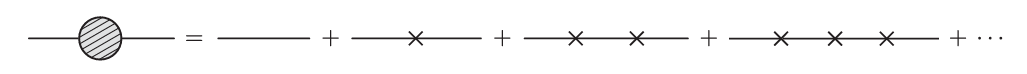
\includegraphics[width=0.8\textwidth]{22.png}
	\caption{two external lines correction}
\end{figure}

Similar proceedure will be excecuted to every single line,if there are multiple of them.The following is a correction term for four external lines Feynman diagram
\begin{figure}[htbp]
	\centering
	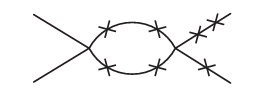
\includegraphics[width=0.7\textwidth]{23.png}
	\caption{four external lines Feynman diagram correction}
\end{figure}

These crosses are interpreted as self-energy,that is,meson-meson interaction.One can imagine the meson flows along the line and somehow interact with vacuum or itself and continues to flow along the line till next cross.Thus these corrections are actually propogations correction of meson.So this cross can also be imagined as some sort of inner loop with momenta flowing along it,which represents self-interaction or vacuum interaction.
\section{mathematical details}
A question necessary to be asked is "what is the contribution of a $\times$ on a line?".Not like regular dot,"$\times$" is caused by $(Z_3-1)[\frac{1}{2}(\partial\phi')^2-\frac{1}{2}m^2\phi'^2]$,which contains not only $\phi'$ but also $\partial_{\mu}\phi'$.If this term only contains $\phi'$,then the regular Feynman rules can be certainly applied,however,there is $\partial_{\mu}\phi'$.The conclusion is that a $\partial^{\mu}(\text{field})$ term will contribute to $\pm ip^{\mu}_{\text{field}}$ in a Feynman diagram

\[
\fbox{%
	$\partial^\mu(\text{field}) \text{ in } \mathcal{L}_I 
	\xRightarrow{ }
	\pm i p^\mu_{\text{field}} \text{ in Feynman rules}$
}
\]

More explicitly,each $\times$ contributed by $(Z_3-1)[\frac{1}{2}(\partial\phi')^2-\frac{1}{2}m^2\phi'^2]$ results in a factor $i(Z_3-1)(2\pi)^4\delta^{(4)}(q_1+q_2)[q_1^2-m^2]$,where $q_1$ and $q_2$ are momenta flowing through this cross.Besides,at each cross,an integral over internal momenta is needed as at the cross,virtual process can equip with all possible momenta.For example,consider the first order,an overall factor is firstly contributed by two bare point,which generate one external line,thus should take up a factor$$(2\pi)^4\delta^{(4)}(q+q')\frac{i}{q^2-m^2}$$
Now turn to the cross,it should contribute to$$\int \frac{d^4 q_1}{(2\pi)^4}i(2\pi)^4\delta^{(4)}(q_1-q)(Z_3-1)(q_1^2-m^2)\frac{i}{q_1^2-m^2}=(1-Z_3)$$Let the series continue,one can eventually find that the correction for a bare line is nothing but a fator $$(1+(1-Z_3)+(1-Z_3)^2+\cdots)=\frac{1}{Z_3}$$\par So the correction rule for $\mathscr{L}=\frac{1}{2}\partial_{\mu}\phi\partial^{\mu}\phi-\frac{1}{2}m^2\phi^2$ to bare line between two vertex is to multiply it by $\frac{1}{Z_3}$.
\section{aside}
To say something more on correction of propogator.A regular propogator in momenta space looks like$$\frac{u}{q^2-m^2}$$,now when cross,thus self-interaction or vacuum interaction is added,it becomes$$\frac{i}{q^2-m^2-\Sigma}$$Expand it to get corrction order by order$$\frac{i}{q^2-m^2-\Sigma}=\frac{i}{q^2-m^2}[1+\frac{\Sigma}{q^2-m^2}+(\frac{\Sigma}{q^2-m^2})^2+\cdots]$$which looks extremtly alike what is discussed above.
\end{document}